% vim:tw=72 sw=2 ft=tex
%         File: HW2.tex
% Date Created: 2016 Feb 11
%  Last Change: 2016 Feb 16
%     Compiler: pdflatex
%       Author: Adam Lang $ Gabriel Anderson Santiago
\documentclass[12pt,a4paper]{article}
\usepackage{amsmath, amssymb}
\usepackage[utf8]{inputenc}
\usepackage[T1]{fontenc}
\usepackage[english]{babel}
\usepackage{graphicx}
\usepackage{float}
\graphicspath{{fig/}}
\usepackage{tikz}

\title{Homework assignment 2 - EL2450}
\author{Adam Lang (861110-3956) \& Gabriel Andersson Santiago
(910706-4538)}

\begin{document}
\subsection{}
The system will become unstable when a delay of 0.4 seconds is used. The settling time for 0.39 is quite long but the system does stabilize. Figure \ref{fig:network_delay} shows different time delay settings in Simulink. It clearly shows that a delay of 0.3 seconds still makes the system stabilize quickly while a delay of 0.4 makes it unstable.

\begin{center}
      \begin{figure}[H]
      \centering
        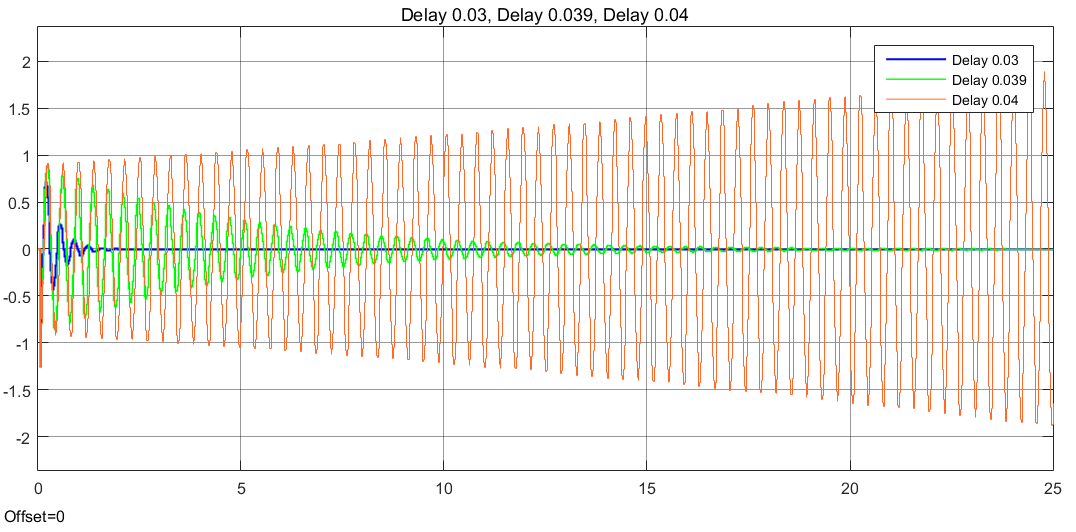
\includegraphics[scale=0.5]{network_delay.png}
        
      \caption{Control signal for different delay settings}
      \label{fig:network_delay}
      
      \end{figure}
    \end{center}
    

\end{document}